
%%%%%%%%%%%%%%%%%%%%%%%%%%%%%%%%%%%%%%%%
%           main body
%%%%%%%%%%%%%%%%%%%%%%%%%%%%%%%%%%%%%%%%


%-----------------------------------
%	TITLE PAGE
%-----------------------------------

\title[Convex Optimization]{\LARGE \bfseries 第四部分\quad 凸优化} % The short title appears at the bottom of every slide, the full title is only on the title page
\author[Convex Sets and Convex Functions] % Your institution as it will appear on the bottom of every slide, may be shorthand to save space
{\Large \bfseries \S 2. 凸集与凸函数}
% \author{Singular Value Decomposition} % Your name
% \date{\today} % Date, can be changed to a custom date
\date{}

%------------------------------------------------

\begin{document}


%------------------------------------------------

\begin{frame}

\titlepage % Print the title page as the first slide

\end{frame}

%------------------------------------------------

\begin{frame}
\frametitle{内容提要} % Table of contents slide, comment this block out to remove it
\tableofcontents % Throughout your presentation, if you choose to use \section{} and \subsection{} commands, these will automatically be printed on this slide as an overview of your presentation
\end{frame}

%-----------------------------------
%	PRESENTATION SLIDES
%-----------------------------------

\section{凸集}

%------------------------------------------------

\begin{frame}

\begin{block}{凸集，Convex Set}
设$C$为$\mathbb{R}^n$的一个子集。如果任取$C$中两点$\mathbf{x}_1, \mathbf{x}_2$, 以这两点为端点的线段包含在集合$C$中，即
\[\theta \mathbf{x}_1 + (1-\theta)\mathbf{x}_2 \in C\]
对任意满足$0\le \theta \le 1$的非负实数$\theta$都成立，则称$C$为$\mathbb{R}^n$中的一个凸集。
\end{block}

\end{frame}

%------------------------------------------------

\begin{frame}

\begin{block}{凸集与非凸集的例子}
\begin{figure}[H]
\begin{minipage}[b]{0.48\textwidth}
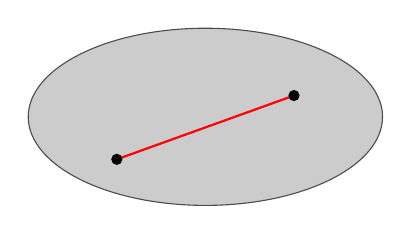
\begin{tikzpicture}[scale=0.45]
\draw[black!70, fill=black!20] (0,0.5) ellipse (5 and 2.5);
\draw[red,thick] (-2.5,-0.7) -- (2.5,1.1);
\filldraw (-2.5,-0.7) circle[radius=4pt];
\filldraw (2.5,1.1) circle[radius=4pt];
\end{tikzpicture}
\caption*{凸集}
\end{minipage} \hfill
\begin{minipage}[b]{0.48\textwidth}
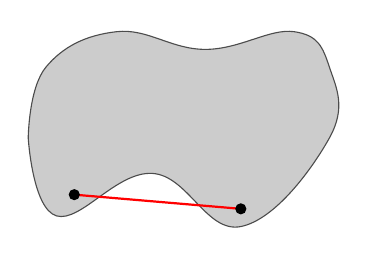
\begin{tikzpicture}[scale=0.45]
\draw[black!70, fill=black!20] plot[smooth, tension=.7] coordinates {(-3.5,0.5) (-3,2.5) (-1,3.5) (1.5,3) (4,3.5) (5,2.5) (5,0.5) (2.5,-2) (0,-0.5) (-2.7,-1.7) (-3.5,0.5)};
\draw[red,thick] (-2.2,-1.1) -- (2.5,-1.5);
\filldraw (-2.2,-1.1) circle[radius=4pt];
\filldraw (2.5,-1.5) circle[radius=4pt];
\end{tikzpicture}
\caption*{非凸集}
\end{minipage}
\end{figure}
\end{block}

\end{frame}

%------------------------------------------------

\begin{frame}

\begin{block}{一些重要的凸集}
\begin{itemize}
\item 超平面（Hyperplane）：$\{\mathbf{x} \ |\ \mathbf{a}^T\mathbf{x} = b\}$
\item 半空间（Halfspace）：$\{\mathbf{x} \ |\ \mathbf{a}^T\mathbf{x} \le b\}$
\item 球（Ball）与椭球（Ellipsoid）：
\[\{\mathbf{x} \ |\ (\mathbf{x} - \mathbf{x}_0)^TP^{-1}(\mathbf{x} - \mathbf{x}_0) \le 1 \}\]
其中$P$是一个正定阵。
\item 范数球（Norm Ball）：$\{\mathbf{x} \ |\ \Vert \mathbf{x} - \mathbf{x}_0 \Vert \le r \}$
\item 多面体（Polyhedra）：
\[\{\mathbf{x} \ |\ \mathbf{a}_i^T\mathbf{x} \le b_i, \mathbf{c}_j^T\mathbf{x} = d_j\}\]
为有限个半空间与超平面的交集。
\end{itemize}
\end{block}

\end{frame}

%------------------------------------------------

\begin{frame}

\begin{block}{凸组合，Convex Combination}
设$\mathbf{x}_1, \ldots, \mathbf{x}_k$为$\mathbb{R}^n$中的$k$个点，称
\[\mathbf{x} = \theta_1\mathbf{x}_1 + \cdots \theta_k\mathbf{x}_k \in \mathbb{R}^n\]
为这$k$个点的一个凸组合，其中$\theta_i \ge 0$且满足$\theta_1 + \cdots + \theta_k = 1$.
\end{block}

\vspace{1em}

\begin{block}{凸包，Convex Hull}
称集合$C\in\mathbb{R}^n$中点的所有的凸组合组成的集合为$C$的凸包，记作$\operatorname{conv} C$, 即
\[\operatorname{conv} C = \left\{ \theta_1\mathbf{x}_1 + \cdots \theta_k\mathbf{x}_k \right\}\]
$k$是正整数，$\mathbf{x}_1, \ldots, \mathbf{x}_k$是$C$中的点，$\theta_i \ge 0$, $\theta_1 + \cdots + \theta_k = 1$. $\operatorname{conv} C$是包含$C$的最小的凸集。
\end{block}

\end{frame}

%------------------------------------------------

\begin{frame}

\begin{block}{凸包的例子}
\begin{center}
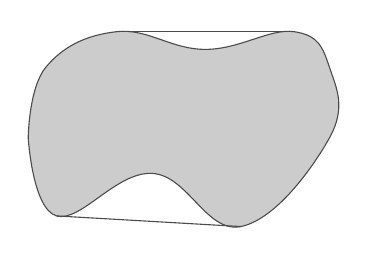
\begin{tikzpicture}[scale=0.45]
\draw[black!70, fill=black!20] plot[smooth, tension=.7] coordinates {(-3.5,0.5) (-3,2.5) (-1,3.5) (1.5,3) (4,3.5) (5,2.5) (5,0.5) (2.5,-2) (0,-0.5) (-2.7,-1.7) (-3.5,0.5)};
% \filldraw (-1,3.5) circle[radius=4pt];
% \filldraw (4,3.5) circle[radius=4pt];
% \filldraw (2.5,-2) circle[radius=4pt];
% \filldraw (-2.7,-2) circle[radius=4pt];
\draw[black!70] (-1,3.5) -- (4,3.5);
\draw[black!70] (2.5,-2) -- (-2.7,-1.7);
\end{tikzpicture}
\end{center}
\end{block}

\end{frame}

%------------------------------------------------

\begin{frame}

\begin{block}{保凸集的运算}
\begin{itemize}
\item 交：若$C_1,C_2$是两个凸集，则$C_1\cap C_2$也是。更一般地，任意多凸集的交仍然是凸集。
\item 仿射（Affine）映射：
\[f: \mathbb{R}^n \to \mathbb{R}^m, \; \mathbf{x} \mapsto A\mathbf{x} + \mathbf{b}\]
凸集在仿射映射下的像与原像都是凸集。
\item 分式线性（Linear Fractional）映射：
\[f: \{ \mathbf{x} \in \mathbb{R}^n \ |\ \mathbf{c}^T\mathbf{x} + d > 0 \} \to \mathbb{R}^m, \; \mathbf{x} \mapsto \dfrac{1}{\mathbf{c}^T\mathbf{x} + d}(A\mathbf{x} + \mathbf{b})\]
\end{itemize}

\end{block}

\end{frame}

%------------------------------------------------

% \begin{frame}

% \begin{block}{}

% \end{block}

% \end{frame}

%------------------------------------------------

\section{凸函数}

%------------------------------------------------

\begin{frame}

\begin{block}{凸函数，Convex Function}
如果一个函数$f: C\to \mathbb{R}$是定义在$\mathbb{R}^n$中的一个凸集$C$上的函数。称$f$是一个凸函数，如果
\[f(\theta\mathbf{x}_1 + (1-\theta)\mathbf{x}_2) \le \theta f(\mathbf{x}_1) + (1-\theta)f(\mathbf{x}_2)\]
对任意的$\mathbf{x}_1, \mathbf{x}_2 \in C$以及任意的满足$0\le\theta\le1$的非负实数$\theta$都成立。
\begin{itemize}
\item 如果上述不等式当$\mathbf{x}_1 \neq \mathbf{x}_2$以及$0<\theta<1$都严格成立，那么称$f$是严格凸的。
\item 如果$-f$是（严格）凸的，那么称$f$是（严格）凹（Concave）的。
\end{itemize}
\end{block}

\end{frame}

%------------------------------------------------

\begin{frame}

\begin{block}{常见凸函数}
\begin{itemize}
\item 仿射函数：$\mathbf{x} \mapsto \mathbf{a}^T\mathbf{x} + b$
\item 范数函数：$\mathbf{x} \mapsto \Vert \mathbf{x} \Vert_p$, 其中$p\ge1$为实数或为$\infty$
\item 最大值函数：$\mathbf{x} \mapsto \max\{x_1,\ldots,x_n\}$
\item 指数函数：$x \mapsto e^{ax}$
\item 幂函数：$x \mapsto x^{a}$, 其中$a \ge 1$或$a\le 0$
% \item
% \item
\end{itemize}
\end{block}

\end{frame}

%------------------------------------------------

\begin{frame}

\begin{block}{判别凸函数的方法}
\begin{itemize}
\item 用定义验证
\item 一阶条件：$f(\mathbf{y}) \ge f(\mathbf{x}) + \nabla f(\mathbf{x})^T(\mathbf{y} - \mathbf{x})$
\item 二阶条件：$f$的黑塞矩阵$H(f)$在所有点都是半正定的
\item 上境图（Epigraph）为凸集
\[\operatorname{epi}f = \{ (\mathbf{x}, t) \ |\ f(\mathbf{x}) \le t \}\]
\item 由凸函数通过保凸运算得到的函数
% \item
\end{itemize}
\end{block}

\end{frame}

%------------------------------------------------

\begin{frame}

\begin{block}{保凸函数的运算}
\begin{itemize}
\item 非负加权求和：$f_1,\ldots,f_m$是凸函数，则
\[f = w_1f_1+\cdots+w_mf_m\]
仍是凸函数，其中$w_1,\ldots,w_m$都是非负实数
\item 取最大值：$f_1,\ldots,f_m$是凸函数，则
\[f(x) = \max\{f_1(x),\ldots,f_m(x)\}\]
仍是凸函数
\item 取上确界（Supremum）：若对每个$\mathbf{y}$, 函数$f(\mathbf{x}, \mathbf{y})$都是$\mathbf{x}$的凸函数，那么
\[g(\mathbf{x}) = \sup\limits_{y} f(\mathbf{x}, \mathbf{y})\]
% \item
% \item
\end{itemize}
\end{block}

\end{frame}

%------------------------------------------------

\begin{frame}

\begin{block}{保凸函数的运算}
\begin{itemize}
\item 复合$f: \mathbb{R}^n \xrightarrow{g = (g_1,\ldots,g_k)} \mathbb{R}^k \xrightarrow{h} \mathbb{R}$, 那么以下条件下，$f$是凸的：
\begin{itemize}
\item[$\bullet$] 每个$g_i$都是凸函数；$h$是凸函数，且$h$对于每一个自变量都是非减函数
\item[$\bullet$] 每个$g_i$都是凹函数；$h$是凸函数，且$h$对于每一个自变量都是非增函数
\end{itemize}

% \item
% \item
\end{itemize}
\end{block}

\end{frame}

%------------------------------------------------

\begin{frame}

\begin{block}{函数的扩展值延伸，Extended-Value Extension}
为了方便，通常对于凸函数$f$的定义域之外的$\mathbf{x}$, 还补充定义其函数值为$+\infty$, 即
\[\widetilde{f}(\mathbf{x}) := \begin{cases}
f(\mathbf{x}), & \mathbf{x} \text{ 在定义域中} \\
+\infty, & \mathbf{x} \text{ 不在定义域中}
\end{cases}\]
并将其称作是$f$的扩展值延伸。

\vspace{1em}

类似地，凹函数的扩展值延伸被定义作
\[\widetilde{f}(\mathbf{x}) := \begin{cases}
f(\mathbf{x}), & \mathbf{x} \text{ 在定义域中} \\
-\infty, & \mathbf{x} \text{ 不在定义域中}
\end{cases}\]
\end{block}

\end{frame}

%------------------------------------------------

\section{共轭函数}

%------------------------------------------------

\begin{frame}

\begin{block}{共轭函数，Conjugate Function}
函数$f: \mathbb{R}^n \to \mathbb{R}$的共轭函数被定义作
\[f^*(\mathbf{y}) = \sup\limits_{\mathbf{x}} \left( \mathbf{y}^T\mathbf{x} - f(\mathbf{x}) \right)\]

\begin{itemize}
\item $f^*$是$\mathbf{y}$的一系列的凸函数的逐点上确界，因此无论$f$是不是凸函数，$f^*$总是凸的。
\end{itemize}
\end{block}

\end{frame}

%------------------------------------------------

\begin{frame}

\begin{block}{共轭函数例子}
\begin{itemize}
\item 负对数函数$f(x) = -\ln x$的共轭为
\begin{align*}
f^*(y) & = \sup\limits_{x>0} \left( xy + \ln x \right) = \begin{cases}
-\ln(-y) - 1, & y < 0 \\
+\infty, & y \ge 0
\end{cases}
\end{align*}
\item 正定二次型$f(\mathbf{x}) = \dfrac{1}{2} \mathbf{x}^T Q \mathbf{x}$的共轭为
\[f^*(\mathbf{y}) = \sup\limits_{\mathbf{x}} \left( \mathbf{y}^T\mathbf{x} - \dfrac{1}{2} \mathbf{x}^T Q \mathbf{x} \right) = \dfrac{1}{2} \mathbf{y}^T Q^{-1} \mathbf{y}\]
\end{itemize}
\end{block}

\end{frame}

%------------------------------------------------
% % closing page
% \begin{frame}
% \HUGE{\centerline{\bfseries {\color{gray} The} {\color{zkblue} End}}}

% \pause

% \vspace{1.2em}

% \Large{\centerline{\bfseries {\color{gray}Thank} \quad {\color{zkblue} You}}}

% \end{frame}

%----------------------------------------------------------------------------------------

\end{document}
